\documentclass[12pt,a4paper]{article}
\usepackage[utf8]{inputenc} % sempre salve seus arquivos como UTF8
\usepackage[T1]{fontenc}
\usepackage[english]{babel}

\usepackage[left=2.5cm,right=2cm,top=2cm,bottom=2.5cm]{geometry}
\usepackage{amsmath}
\usepackage{amsthm}
\usepackage{amsfonts}

\usepackage{graphicx}
\usepackage{algorithm}
\usepackage{color}
\usepackage[noend]{algpseudocode}
\usepackage{mathtools}
\usepackage{subfig}
\usepackage{diagbox}

% load times font
\usepackage{mathptmx}
\usepackage[scaled=.90]{helvet}
\usepackage{courier}

% comandos
\newcommand{\mdc}[1]{\mathrm{mdc}(#1)}

\DeclarePairedDelimiter\ceil{\lceil}{\rceil}
\DeclarePairedDelimiter\floor{\lfloor}{\rfloor}

% Foot without marker
\newcommand\blfootnote[1]{%
	\begingroup
	\renewcommand\thefootnote{}\footnote{#1}%
	\addtocounter{footnote}{-1}%
	\endgroup
}

\title{MO446 -- Introduction to Computer Vision  \\ Project 2}
\author{Breno Leite  \\ Guilherme Leite}
\date{19/09/2017}

\begin{document}

\maketitle
\blfootnote{\textit{\textbf{Important note:} The borders seen in the figures are not part of the image, they are figurative information about the starting and ending points of the image. Moreover, all the image scales in this report were changed in order to make the text more readable.}} \\

%% ---------------- Starts here --------------------------------

\textbf{\LARGE Input Video}\\

	A video can be seeing as nothing more than a sequence of frames showed in a specific frequency to illude the human eye into perceiving movement, imitating the human vision. With this knowledge in mind it is feasible to abstract the problem of stabilizing an entire video into several sub-problems of stabilizing a pair of video frames at a time. This approach enables the experiments results to be presented in form of images, moving the video output to the very end of the report.
\par
	The sub-problems experiements that compose the solution were performed on Figure \ref{fig:inputFigureSub} and Figure \ref{fig:inputFigureClut}.

\begin{figure}[!h]
	\centering
	\subfloat[Sub image to be found in cluttered environment (\textbf{p2-2-0})]{
		{
			\setlength{\fboxsep}{1pt}
			\setlength{\fboxrule}{1pt}
			\fbox{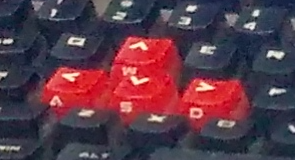
\includegraphics[scale=0.5]{debug/input1}}
		}
		\label{fig:inputFigureSub}
	}
	\quad
	\subfloat[Cluttered environment (\textbf{p2-2-1})]{
		{
			\setlength{\fboxsep}{1pt}
			\setlength{\fboxrule}{1pt}
			\fbox{\includegraphics[scale=0.08]{debug/input2}}
		}
		\label{fig:inputFigureClut}
	}
	\caption{Initial images used on the experiments.}
	\label{fig:inputFigure}
\end{figure}

\textbf{\LARGE Question 3 - Video Stabilization Algorithm}\\

\textbf{3.1 )} The SIFT descriptor was chosen to find the interest points and descriptors, we couldn't fully implement it due to the density of details, misleading information, time constrains and complex concepts. Since the remaining of the project requires SIFT's output we opted to use OpenCV implementation of the SIFT descriptor on the following questions.
\par
The SIFT descriptor has mainly two independent operations: detection of interest points, also called key points by Lowe, and extraction of a descriptor for each key point.

\begin{figure}[!h]
	\centering
	\subfloat[Keypoints in sub image (\textbf{p2-3-1-0})]{
		{
			\setlength{\fboxsep}{1pt}
			\setlength{\fboxrule}{1pt}
			\fbox{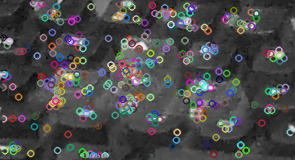
\includegraphics[scale=0.5]{report/p2-3-1-0}}
		}
		\label{fig:keypointsSub}
	}
	\quad
	\subfloat[Keypoints in cluttered image (\textbf{p2-3-1-1})]{
		{
			\setlength{\fboxsep}{1pt}
			\setlength{\fboxrule}{1pt}
			\fbox{\includegraphics[scale=0.08]{report/p2-3-1-1}}
		}
		\label{fig:keypointsClut}
	}
	\caption{Keypoints found by the SIFT descriptor.}
	\label{fig:keypoints}
\end{figure}

	In Figure \ref{fig:keypoints} all the key points in the image are shown in coloured circles. To detect these key points the algorithm creates a so called scale space which can be seem as a matrix, its columns are called octaves and its rows are called scales. The first octave consists of the original image and it is gradually blurred, by a factor of $sigma$, as the scales increase, the first image of the next octave is a subsample of the first image in the current octave, in our partial implementation the image is subsampled by half its size, along with the octaves and scales creation a Difference of Gaussian (DoG) is also generated. The difference of gaussian is generated within each octave and is done by the subtraction between two consecutive scales, the result is a black image with white spots denoting the edges in the image. With the DoG, for each octave, in hands a pre selection of the key points is executed, for every DoG in every octave, select a pixel and check its intensity against its neighbourhood in its scale and also in the above and below scales, if the select pixel is the greater or the lowest of all points, then it is a approximation of a key point, this is also as far as we got to implement SIFT in our code, the actual key point position is found with by the Taylor expansion. Of all the key points generated in the last step many of them are false positives, so they are filtered out. To remove the low contrast points a threshold is used on the point intensity, the threshold value to be used would be of 0.03 according to Lowe, but further testing would be needed to make sure it fits our data. To remove edges and keep the corners a second filter must be done, at each key point two gradients are calculated perpendicular to each other, in a corner both gradients would be big, since corners are key points they are kept and the rest is discarded, the threshold is done on the ratio between the two eigenvalues and its value is recommended of 5 by Lowe, at the end of the filtering only the actual key points remain.
\par
	Before extracting the descriptors for each key point the algorithm ensures rotation invariance by setting a rotation for each key point. A gradient magnitude and orientation is calculated for every pixel around the key point, a histogram of orientations is created discretizing the orientation angles into 36 bins, the amount to be added is proportional to the magnitude of the gradient at that point, the size of the surrounding to be analyzed is based on the gaussian kernel by a factor of $sigma$. To extract the descriptors a area of 16x16 pixels around the key point is taken in consideration, this area is divided again in 4x4 areas and within this area gradient orientation and magnitude are calculated weighted with a gaussian weight function, discretized to a histogram of 8 bins. This will result on 128 values, gathered in a feature vector, that are normalized and now describe that single key point.

\textbf{3.2 )} At this point the SIFT transform has given back all the key points it has found in both images, as seen in Figure \ref{fig:keypoints}, and all the descriptors also found in both images. But still there is no relation between the key points in Figure \ref{fig:keypointsSub} and the ones in Figure \ref{fig:keypointsClut}, and to relate those key points a matching process is performed.
\par
	The goal of the matching is to find the same descriptor, or the closest ones, in both Figure \ref{fig:keypointsSub} and Figure \ref{fig:keypointsClut}. To do so an euclidian distance is calculated between any two descriptors, one in each image, and if they are the same then the distance result will be minimal. The distance is calculated between every descriptor in Figure \ref{fig:keypointsSub} and every descriptor in Figure \ref{fig:keypointsClut}.

\begin{figure}[!h]
	\centering
		{
			\setlength{\fboxsep}{1pt}
			\setlength{\fboxrule}{1pt}
			\fbox{\includegraphics[scale=0.1]{report/p2-3-2-0}}
		}
	\caption{Matching process ignoring ratios (p2-3-2-0)}
	\label{fig:noRatio}
\end{figure}
	
	This algorithm isn't perfect, as seen in Figure \ref{fig:noRatio}, some false positives arise because a key point might have a similar one in a far away position of the image, this is common in images with repeating structures, to eliminate these incorrect relations a new filtering occurs, additional to the closest descriptor match, the second closest descriptor is also retrieved and a ratio between both is calculated, if the ratio between both is greater than a threshold the relation is ignored. In his article Lowe suggests a ratio of 0.8 but it didn't performed well with our data, so we used a 0.75 value.

\begin{figure}[!h]
	\centering
	\subfloat[Ratio of 0.90 (\textbf{p2-3-2-1})]{
		{
			\setlength{\fboxsep}{1pt}
			\setlength{\fboxrule}{1pt}
			\fbox{\includegraphics[scale=0.1]{report/p2-3-2-1}}
		}
		\label{fig:ratio90}
	}
	\quad
	\subfloat[Ratio of 0.75 (\textbf{p2-3-2-2})]{
		{
			\setlength{\fboxsep}{1pt}
			\setlength{\fboxrule}{1pt}
			\fbox{\includegraphics[scale=0.1]{report/p2-3-2-2}}
		}
		\label{fig:ratio75}
	}
	\caption{Ratio between descriptors distance experiments.}
	\label{fig:matchRatio}
\end{figure}

	Figure \ref{fig:matchRatio} shows the difference between thresholds. Figure \ref{fig:ratio90} shows that at ratio 0.9 the filter still allows some false positives to go through, and Figure \ref{fig:ratio75} at ratio 0.75 was the best result we had before the filter started cutting out correct matches, according to Lowe a ratio of 0.8 should eliminate 90\% of false matches and discard only 5\% of the correct ones. We also performed a sandbox experiment, Figure \ref{fig:noRatio} ignoring ratios completely, as expected there are many false positives matches because of these points neighbourhoods. We believe that our results difference from Lowe's are caused by distinct cameras and scenes, the keyboard has too many repeating structures that confuses the algorithm.
\par
	We also computed the runtime difference between two implementations of our algorithm, one using a list as data structure to keep all the key points and thus running over the entire list at every check, and the second one using a tree structure performing a searching in a tree structure on every check. The results can be seem in Table \ref{table:match}, it is noticeable how faster the tree structure is specially when dealing with big images, that is because it doesn't need to check every node in the tree to find the best match.

\begin{table}[!h]
	\centering
	\begin{tabular}{|c|c|c|c|}
		\hline
		& \multicolumn{3}{c|}{\textbf{Time (seconds)}} \\ \hline
		\backslashbox{\textbf{Images Size}}{\textbf{Data Structure}}    & \textbf{List}         & \textbf{Tree}          & \textbf{-1}      \\ \hline
		\textbf{160x295 | 1836x3264}  & 67.4      & 13.95      & -1     \\ \hline
		\textbf{50x50 | 500x501} & 0.1485      & 0.0589       & -1     \\ \hline
	\end{tabular}
	\caption{Comparison between our implementation of the matching with a list and a tree structure.}
	\label{table:match}
\end{table}

\textbf{3.3 )} To define the number of iterations before the RANSAC returns the trained parameters we tested with different parameters and used the ones with best results, in this situation 100 iterations showed the best fitting. In out implementation the training is done using three random points due to their results, increasing the sample points CAUSED SOMETHING the algorithm and decreasing it CAUSED ANOTHER SOMETHING. The matrix $A$ is obtained from these samples and is used on all the remaining points, the error from these new tests are accumulated and later used to choose the best fitting model, this values are called affine parameters.
\par
\textbf{3.4 )} Once the affine parameters were defined they are used in our project to transform the video frame $i + 1$ in relation to the frame $i$, the transformation on these frames can cause them to extrapolate the borders of the video window, when this is the case the frame is cut and the empty space left by it is left with black pixels, solutions as zoom in the video so there would be no empty space or zoom out so the frame wasn't occluded and were left aside to facilitate de implementation.

\end{document}
